\documentclass[a4paper,twoside]{report} % for a report (default)

\usepackage{bftn,color} % You need this
\usepackage{subfig}
\usepackage{listings}
\usepackage{verbatim}
\usepackage{tabularx}


\title{Barrelfish OS Services}   % title of report
\author{Team Barrelfish}	% author
\tnnumber{012}  % give the number of the tech report
\tnkey{Barrelfish Services} % Short title, will appear in footer

% \date{Month Year} % Not needed - will be taken from version history

%% \newcommand{\note}[1]{}
\newcommand{\note}[1]{[\textcolor{red}{\textit{#1}}]}

\begin{document}
\maketitle

%
% Include version history first
%
\begin{versionhistory}
\vhEntry{1.0}{20.08.2010}{kuzi}{Initial version}
\end{versionhistory}

% \intro{Abstract}		% Insert abstract here
% \intro{Acknowledgements}	% Uncomment (if needed) for acknowledgements
% \tableofcontents		% Uncomment (if needed) for final draft
% \listoffigures		% Uncomment (if needed) for final draft
% \listoftables			% Uncomment (if needed) for final draft



%%%%%%%%%%%%%%%%%%%%%%%%%%%%%%%%%%%%%%%%%%%%%%%%%%%%%%%%%%%%%%%%%%%%%%%%%%%%%%%%

\chapter{Barrelfish OS Services}\label{chap:services}

\section{Introduction}\label{sec:intro}

Barrelfish is a multi-server OS, which means that any OS based on
Barrelfish will consist of a collection of mutually dependent
services.  Each of these services provides some functionality required
for the OS.

In Barrelfish, a service can be implemented as a single-dispatcher
domain, a multi-dispatcher domain, multiple domains, one or more
libraries, or some combination of these.

In this document we review the services that will make up the base
building blocks of a Barrelfish OS.  After introducing the services,
we discuss dependencies between the services, and then the current
implementation status of each service.

%% Need to get terminology straight.
%% terminology:
%% - process
%% - thread
%% - dispatcher
%% - domain
%% - entity
%% - principal
%% - subject
%% - object


\section{Services}\label{sec:services}

The specific services we've identified are (presented in alphabetical order):

\begin{itemize}
  \item Binding
  \item Capability Management
  \item Debugging
  \item Device Driver
  \item Device Management
  \item Environment
  \item Group Communication
  \item Locking
  \item Memory Allocation
  \item Naming
  \item Network Stack
  \item Power Management
  \item Principals
  \item Process Management
  \item Resource Accounting and Management
  \item Routing
  \item Shell
  \item SKB
  \item Storage Management
  \item Terminal
  \item Threading
  \item Tracing
  \item Virtual Machine Monitor
  \item Virtual Memory
\end{itemize}

\subsection{Binding}

% Category: Communication

The binding service facilitates communication in the system, allowing
dispatchers to export interfaces through endpoints, and enabling other
threads of execution to connect to dispatchers through endpoints.
The binding service also implements the inter-dispatcher communication
mechanisms allowing threads to send messages over connections.

% FIXME: This last bit is strange, however, this definition of the binding
% service includes the communication facilities.  It could also be
% defined as only providing the functionality of connecting the two
% sides, but leaving the communication to another service.

% who is responsible for sending caps? binding or cap management?

\subsection{Capability Management}

% Category: Capability Management

The capability management service provides the functionality to manage
capabilities outside the kernel.  It provides the ability to allocate
space for and create new capabilities, as well as to manipulate them
by moving, copying, and destroying them.  It also implements the
functionality necessary to transfer capabilities between cores, and to
manage and invoke remote capabilities.


\subsection{Debugging}

% Category; Tracing and Debugging

The debugging service provides the functionality to access and
manipulate system memory, and control execution of the system.  It may
provide these services at a minimal level, or provide higher level
services that allow control of system abstractions such as
capabilities, dipatchers, domains, and threads (for example by
attaching to and controlling specific threads).


\subsection{Device Driver}

% Category: Devices

A device driver service provides access and control over a specific
device.  A device driver manages access to device hardware as well as
handling interrupts and other device events.  The devices managed by
device drivers inlcude IO devices, as well as internal devices such as
busses, timers, etc.

\subsection{Device Management}

% Category: Devices

The device management service stores and manages information about
devices in the system. Its responsibilities include collecting such
information, making it available to others, and implementing policy
relating to device initialisation, startup, shutdown, power management, etc.

\subsection{Environment}

% Category: Process Management

The environment service provides an execution environment to threads
of execution. Examples of this are environment variables.

% Andrew says: ``terminal, etc.''

\subsection{Group Communication}

% Category: Communication

The group communication service provides facilities for multicast
commuincation within groups.  It will provide group management, as
well as management of delivery trees, and the mechanisms for message
delivery and reception (including impementation of necessary consensus
protocols). 

\subsection{Locking}

% Category: Synchronisation

The locking service provides facilities and primitives for mutual
exclusion and synchronisation.  This includes implementation of locks,
condition variables, semaphores, etc.  It also involves managing
excution threads to block and wake them as necessary.

\subsection{Memory Allocation}

% Category: Capability Management

The memory allocation service manages physical memory (using
capabilities).  It processes requests for memory, allocating appropriate
memory, and freeing it when necessary. It tracks which memory is in
use, and which memory is free and can be reused.

% typically this service will only be used by:
% services that manipulate virtual memory (managing address spaces, etc.)
% setup shared memory (communication, etc.)
% do capability management

\subsection{Naming}

% Category: Communication

The naming service provides a name space and a name/value mapping
database that allows entries to be added or retreived.  It is largely
used in communication for finding registered services.  It also
supports notification of new entries and changed entries, and a
blocking lookup.

\subsection{Network Stack}

% Category: Interaction and IO

The network stack implements network protocols. It works
together with a networking device. It may provide further surfaces
such as packet filtering, packet instpection, etc.

\subsection{Power Management}

% Category: Resource Management and Accounting

The power management services monitors power usage in the system,
reacts to power-related events, and can manipulate system resources to
control power usage.  It also manages system sleep and wakeup, and
can manipulate subsystems and hardware according to its policy.

\subsection{Principals}

% Category: Protection and Security

The principals service provides the concept of principals in the
system (e.g., accounts, users, process ids, etc.).  The principals are used for
access control, that is, access control policies can be defined in
terms of principals' access to objects.  This service can also provide
authentication functionalities, to authenticate principals'
identities, as well as management of principles (e.g., account control).

\subsection{Process Management}

% Category: Process Management

The process management service provides functionality to create,
manipulate, and manage dispatchers and domains. It may provide a
conventional process abstraction based on the Barrelfish primitives,
or deal with the primitives themselves.  The functionality provided
includes creating, starting, stopping, and pausing processes, as well
as mechanisms for loading processs, and migrating processes.  Part of
process creation and management involves setting up and managing
address spaces.

% FIXME: It is unclear whether this service should also be responsible
% for dispatchers and domains, or whether these (dispatcher and
% domain) should be in a separate service.


\subsection{Resource Accounting and Management}

% Category: Resource Management and Accounting

The resource accounting and management service provides mechanisms to
monitor resource usage, keep accounting, and manipulate resource
usage.  Resources include basic resources such as CPU, memory, and IRQs,
as well as OS resources such as devices, files, network bandwidth,
etc. Manipulating resource usage includes scheduling processes,
scheduling IO operations, throttling network traffic, etc. 

\subsection{Routing}

% Category: Communication

The routing service supports communication between entities that are
not directly connected.  The service is responsible for determining
(intra-machine) routes between the entities, as well as sending the
messages over the communication network, and reserving sufficient
resources over the routes to be able to provide performance and
reliability guarantees.

\subsection{Shell}

% Category: Shell

The shell service provides a command interpreter and task launcher.
It provides an interface for dynamically starting, stopping, and
manipulating system tasks. Note that this is not limited to a
traditional command-line console.

\subsection{SKB}

% Category: SKB

The system knowledge base service provides a database for storing
information about the system (including available hardware, properties
of the hardware, configuration, running services, etc.).  It also
provides an interface for querying the database, as well as for
running complex analysis (e.g., constraint solving) of the data stored
within. 

\subsection{Storage Management}

% Category: Interaction and IO

The storage management service manages the system's storage
infrastructure and provides abstractions for persistent storage.  This
could be in the form of a file system, a database, or something
completely different.

\subsection{Terminal}

% Category: Interaction and IO

The terminal service provides a terminal abstraction that provides
programs with input and output.  A terminal typically multiplexes
output from different programs to a single output destination and
demultiplexes a single source of input among multiple programs.
The terminal service implements the terminal abstraction, and provides
mechanisms for multiplexing multiple terminals.

\subsection{Threading}

% Category: Process Management

The threading service provides a thread model and thread manipulation
functionality. This allows thread manipulation (creation, destruction,
suspend, wakeup, etc.), thread scheduling and thread local storage. 

\subsection{Tracing}

% Category: Tracing and Debugging

The tracing service collects tracing information and makes it
available to analysis and display applications.  The service allows
running entities in the system to log traces with it as well as to
query it about these traces.  Such a service can be used for logging
system events, debugging information, error events, etc.  The tracing
service can also actively monitor the system, and dynamically query
system entities based on queries.  It can also provide notification
functionality to notify entities when given events occur.

\subsection{Virtual Machine Monitor}

% Category: Virtualisation

The virtualisation service provides a virtual machine monitor that
enables guest software (typically an OS) to be run on virtual hardware.
The service manages the loading and unloading of the guest software,
manages emulation of sensitive and privileged instructions and
hardware, and manages the virtualised memory.

\subsection{Virtual Memory}

% Category: Virtual Memory Management

The virtual memory management service manages the system's virtual
memory (by manipulating Barrelfish vnodes and memory caps).  It
provides functionality to map and unmap pages, manage mapping of
device memory, and the creation and manipulation of address spaces.
It is also responsible for paging and swapping.
	

\section{Service Categories}\label{sec:categories}

% probably better to subdivide the services that are too broad
% categories, and just have the fundamental/general categorisation.
% eg.
% capabilities: cap management, memory management, vm? 
% devices: driver, management
% communication: basic, binding, group, routing
% protection: prinicipals, access control
% process: process, threading, environment
% resource managment: resource mgmt and accounting, power mgmt,
% scheduling
% tracing and debugging: tracing, debugging
% these could be used for a layering view...

The above services can be grouped into two categories, depending on
what they are used for in the system.  Roughly, we distinguish between
services that provide key Barrelfish functionality, and services that
provide more general OS functionality.

\subsection{Fundamental Barrelfish Services}

\begin{itemize}
  \item Binding
  \item Capability Management
  \item Group Communication
  \item Naming
    % this is an issue because
    % the naming service is a fundamental BF service for communication
    % it is also a general service in an OS
  \item Process Management
    % this is an issue since there is the aspect of 
    % dispatchers and domains which is BF specific
    % process accounting, process starting, stopping, etc. which is general
  \item Routing
  \item SKB
\end{itemize}

\subsection{General OS Services}

\begin{itemize}
  \item Debugging
  \item Device Driver
  \item Device Management
  \item Environment
  \item Locking
  \item Memory Allocation
    % this is an issue since there is the aspect of
    % dealing with ram caps and bookkeeping which is BF specific 
    % policy and accounting is general
  \item Network Stack
  \item Power Management
  \item Principals
  \item Resource Accounting and Management
  \item Shell
  \item Storage Management
  \item Terminal
  \item Threading
    % this is an issue since there is the aspect of
    % thread scheduling, and implementation which is BF specific
    % thread API, accounting, management, scheduling which is general
  \item Tracing
  \item Virtual Machine Monitor
  \item Virtual Memory
    % this has an issue since there is the aspect of managing vnodes,
    % which is BF specific,
    % the aspect of address space layout, creating and tearing down
    % address spaces, which is a mix between BF specific and general,
    % the aspect of paging, which is general
\end{itemize}



%% \subsection{Fundamental Barrelfish Services}

%% \begin{description}
%%   \item[Capability Management] services that manage capabilities,
%%     including allocation, physical memory management, cpability
%%     transfer, etc. 
%%   \item[Virtual Memory Management] services that manage virtual memory
%%     to provide address spaces, protection, etc. 
%%   \item[SKB] services related to the system knowledge base, including
%%     gathering, storing, and querying system data. 
%%   \item[Communication] services that enable communication within the
%%     system.
%%   \item[Process Management] services related to managing execution in
%%     the system, this includes basic dispatcher and domain
%%     functionality and scheduling, threading within dispatchers, as
%%     well as process accounting, environments, etc. 
%% \end{description}

%% \subsection{General OS Services}

%% \begin{description}
%%   \item[Synchronisation] services that enable threads to synchronise,
%%     including locking and signalling mechanisms. 
%%   \item[Devices] services related to device access, including
%%     interrupt handling, device memory and register access, (PCI) bus
%%     management, device management (starting, stopping, etc.), device
%%     drivers, etc. 
%%   \item[Resource Management and Accounting] services that monitor
%%     resource usage, keep accounting, and make changes to the resource
%%     usage. 
%%   \item[Protection and Security] services that enable and manage
%%     resource monitoring and usage. This includes monioring and
%%     accounting mechanisms, as well as scheduling, power management,
%%     and paging. 
%%   \item[Protection and Security] services that provide mechanisms and
%%     policy for access control. 
%%   \item[Interaction and IO] services that manage the systems external
%%     interaction.  This is at a higher level than device drivers, and
%%     involves abstractions such as filesystems, network stacks, audio
%%     frameworks, etc. 
%%   \item[Shell] services that provide program launching facilities. 
%%   \item[Vitualisation] services that enable virtualisation such as
%%     virtual machine monitors. 
%%   \item[Tracing and Debugging] services that enable collection of
%%     runtime information as well as runtime debugging.  This includes
%%     trace collection and analysis, stubs to access and manipulate
%%     system memory and execution, etc. 
%%   \item[Applications] applications and services that are not typically
%%     considered core OS services. 
%% \end{description}



%%%%%%%%%%%%%%%%%%%%%%%%%%%%%%%%%%%%%%%%%%%%%%%%%%%%%%%%%%%%%%%%%%%%%%%%%%%%%%%%

\chapter{Service Dependencies}\label{chap:dependencies}

The above services are system building blocks and do not operate in
isolation but make use of each other's services.
This leads to dependencies between the various services.

We distinguish between several types of dependencies.
\begin{itemize}
  \item Fundamental dependencies: dependencies that exist due to
    the service's required functionality (e.g., network stack relies on
    the ethernet device driver).
  \item Implementation dependencies: dependencies that exist due
    to implementation details.  This can be further subdivided into:
    \begin{itemize}
      \item dependencies due to being implemented as communicating
        Barrelfish dispatchers (e.g., network stack relies on binding
        because it needs to communicate with the ethernet device
        driver).
      \item dependencies due to specific implementation decisions
        (e.g., network stack using the locking service because it is
        multithreaded).
    \end{itemize}
\end{itemize}

%% there are also dependencies that are due to:
%% - being implemented on a barrelfish system, but related to fundamental design (e.g., device driver using capability management to get access to device hardware)



\section{Dependencies}\label{chap:dependencies}

All the dependencies between the specific services are shown in
Figure~\ref{fig:dep2-a}.

\begin{figure}[hbt]
 \begin{center}
 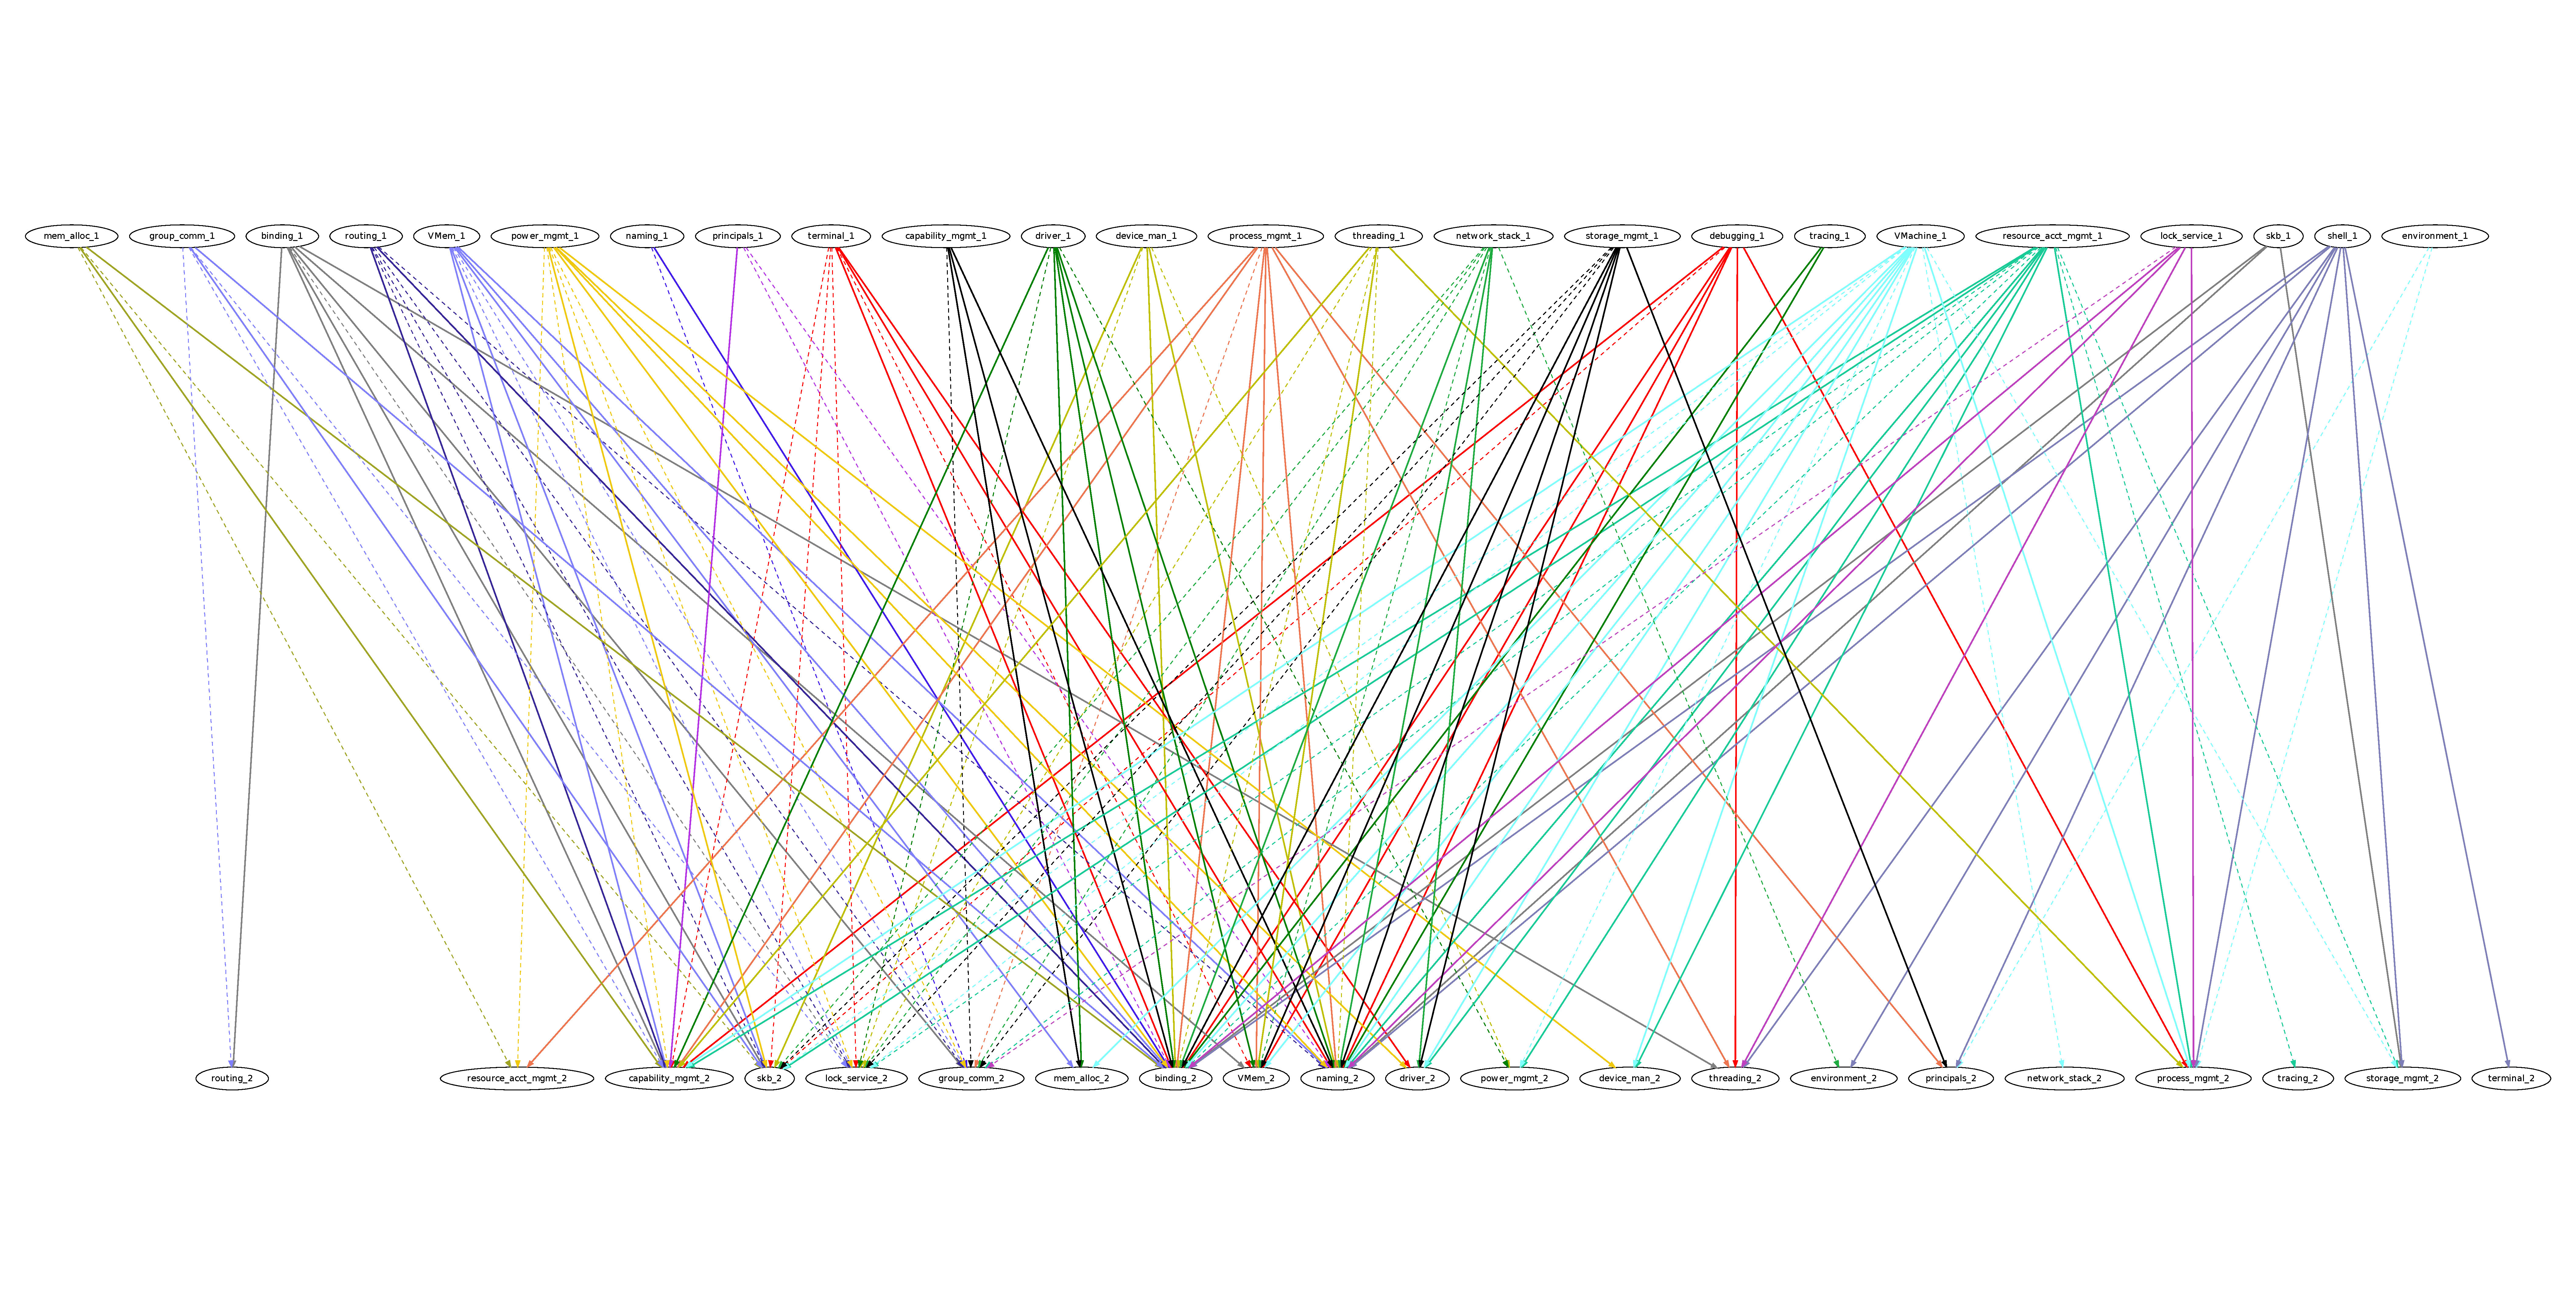
\includegraphics[angle=270,scale=0.15]{dep2-a-dot.pdf}
% \includegraphics[angle=90,width=\columnwidth]{dep2.pdf}
 \end{center}
 \caption{Use dependencies between OS services. Dashed lines indicate
   dependencies we are uncertain about.}\label{fig:dep2-a}
\end{figure}

The subset of fundamental dependencies are shown in
Figure~\ref{fig:dep2-f}. Likewise the subset of implementation
dependencies are shown in Figures~\ref{fig:dep2-b} and~\ref{fig:dep2-i}.

\begin{figure}[hbt]
 \begin{center}
 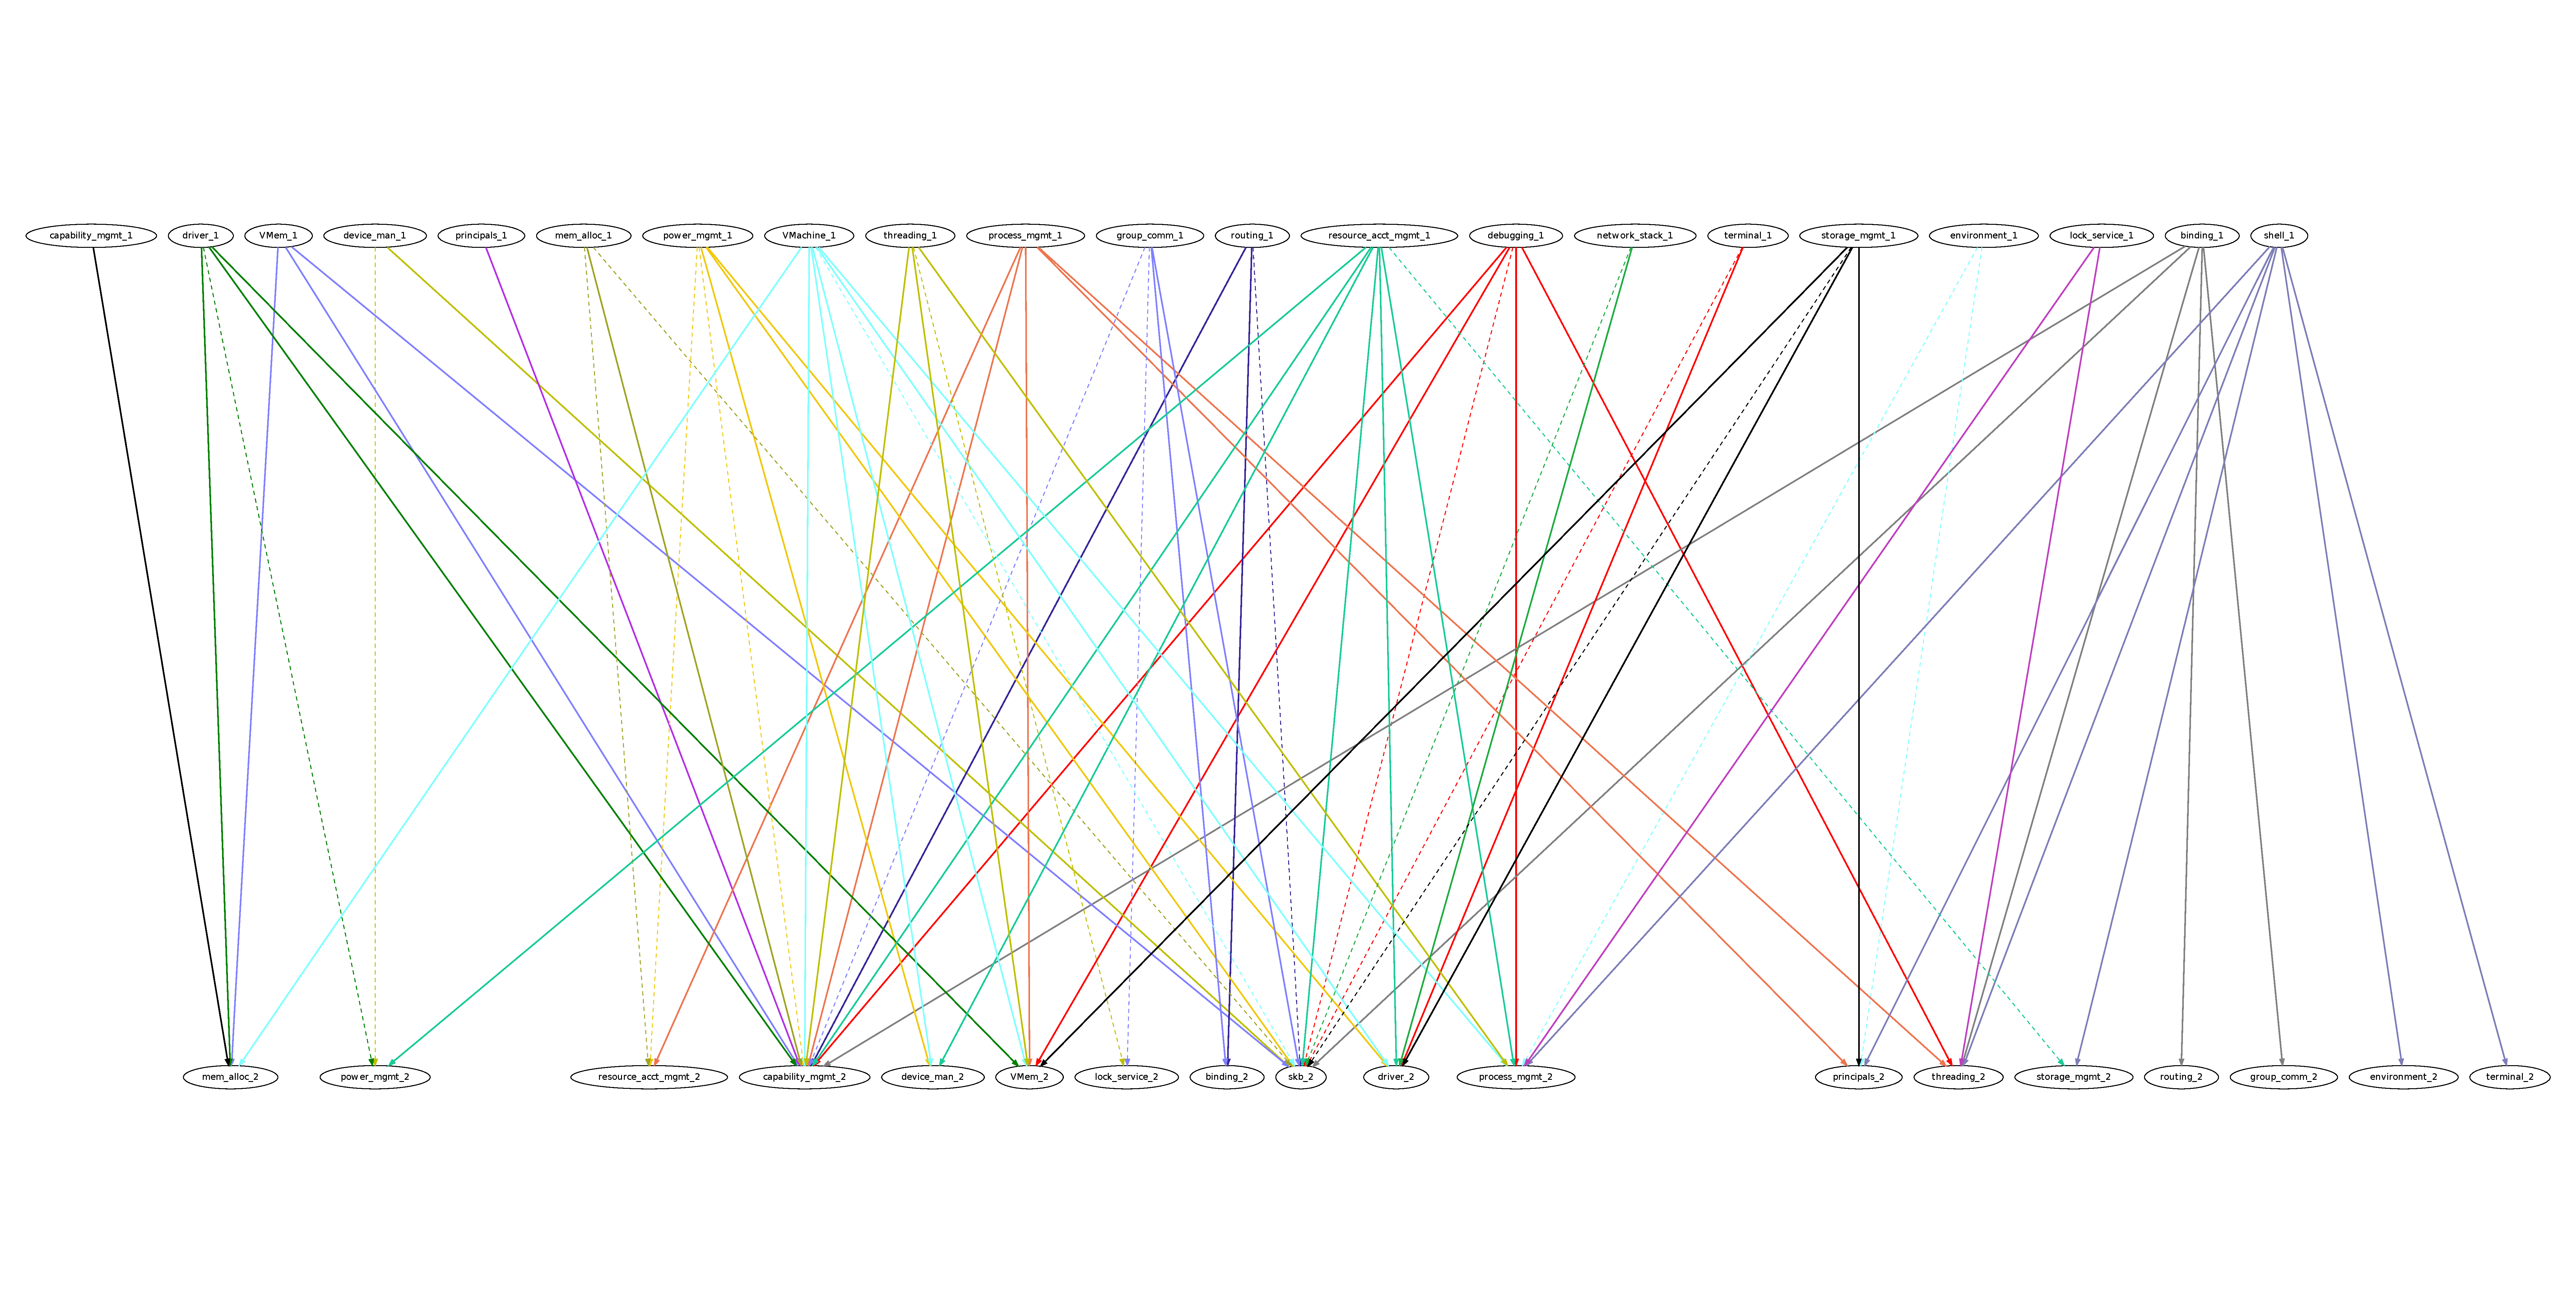
\includegraphics[angle=270,scale=0.15]{dep2-f-dot.pdf}
 \end{center}
 \caption{Subset of fundamental use dependencies between OS
   services.}\label{fig:dep2-f}  
\end{figure}


\begin{figure}[hbt]
 \begin{center}
 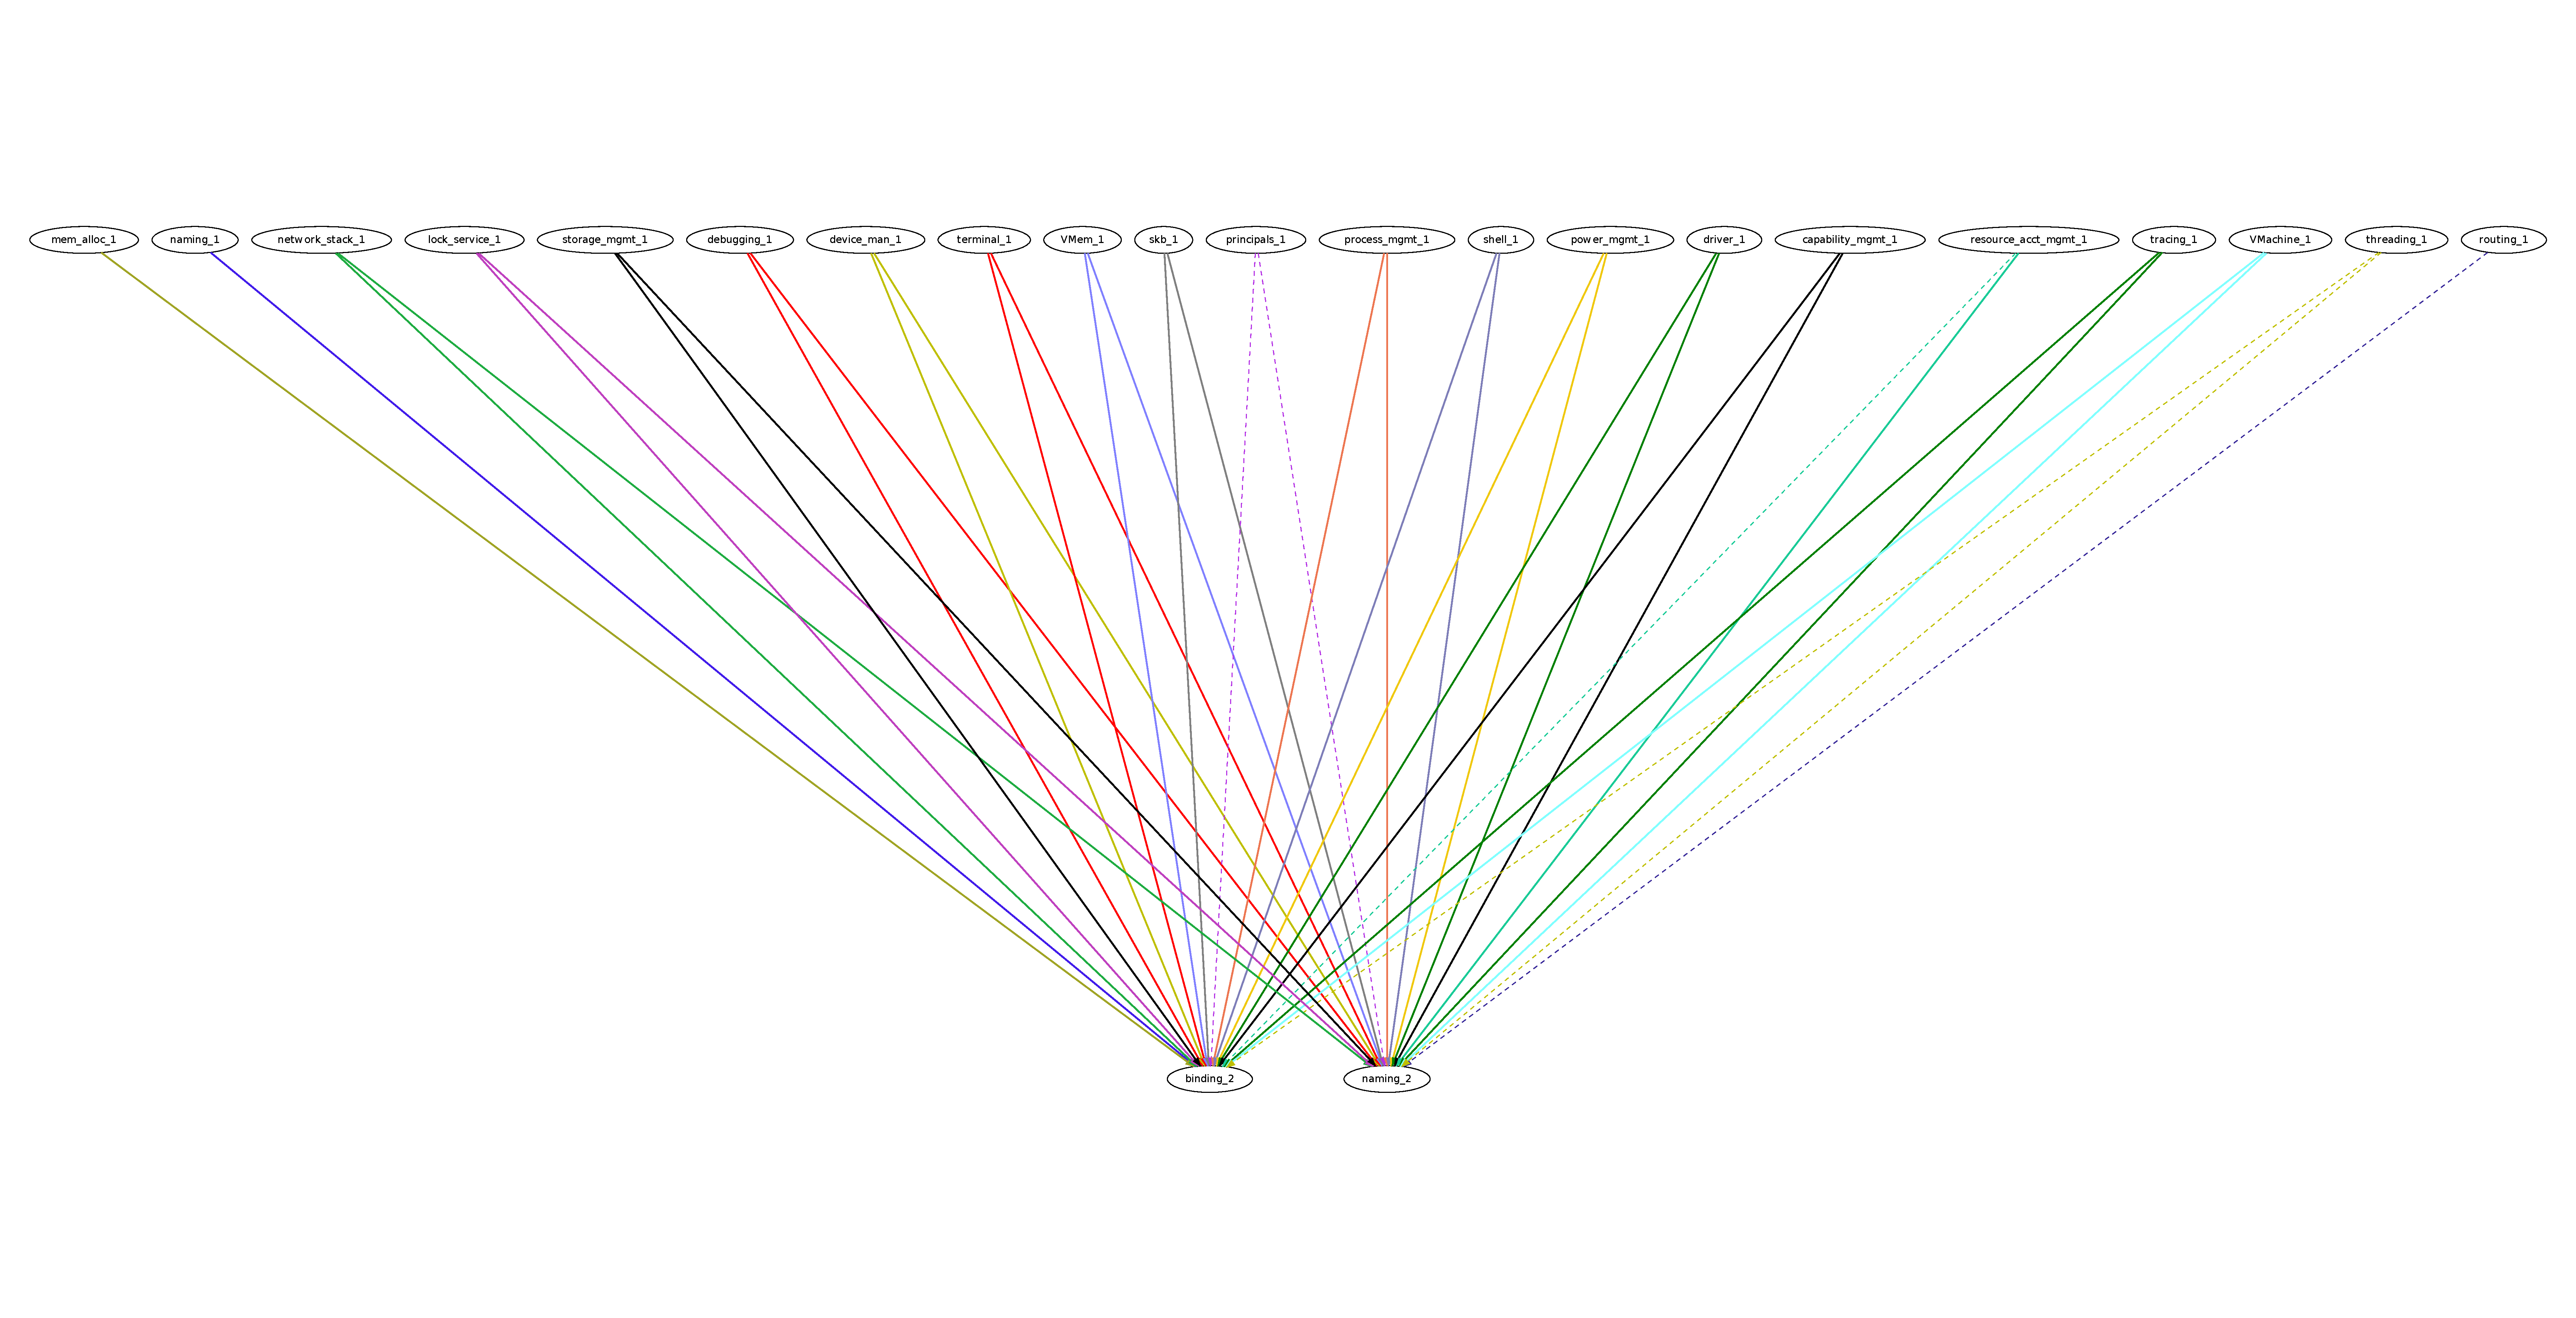
\includegraphics[angle=270,scale=0.15]{dep2-b-dot.pdf}
 \end{center}
 \caption{Subset of barrelfish-implementation specific use
   dependencies between OS services.}\label{fig:dep2-b} 
\end{figure}


\begin{figure}[hbt]
 \begin{center}
 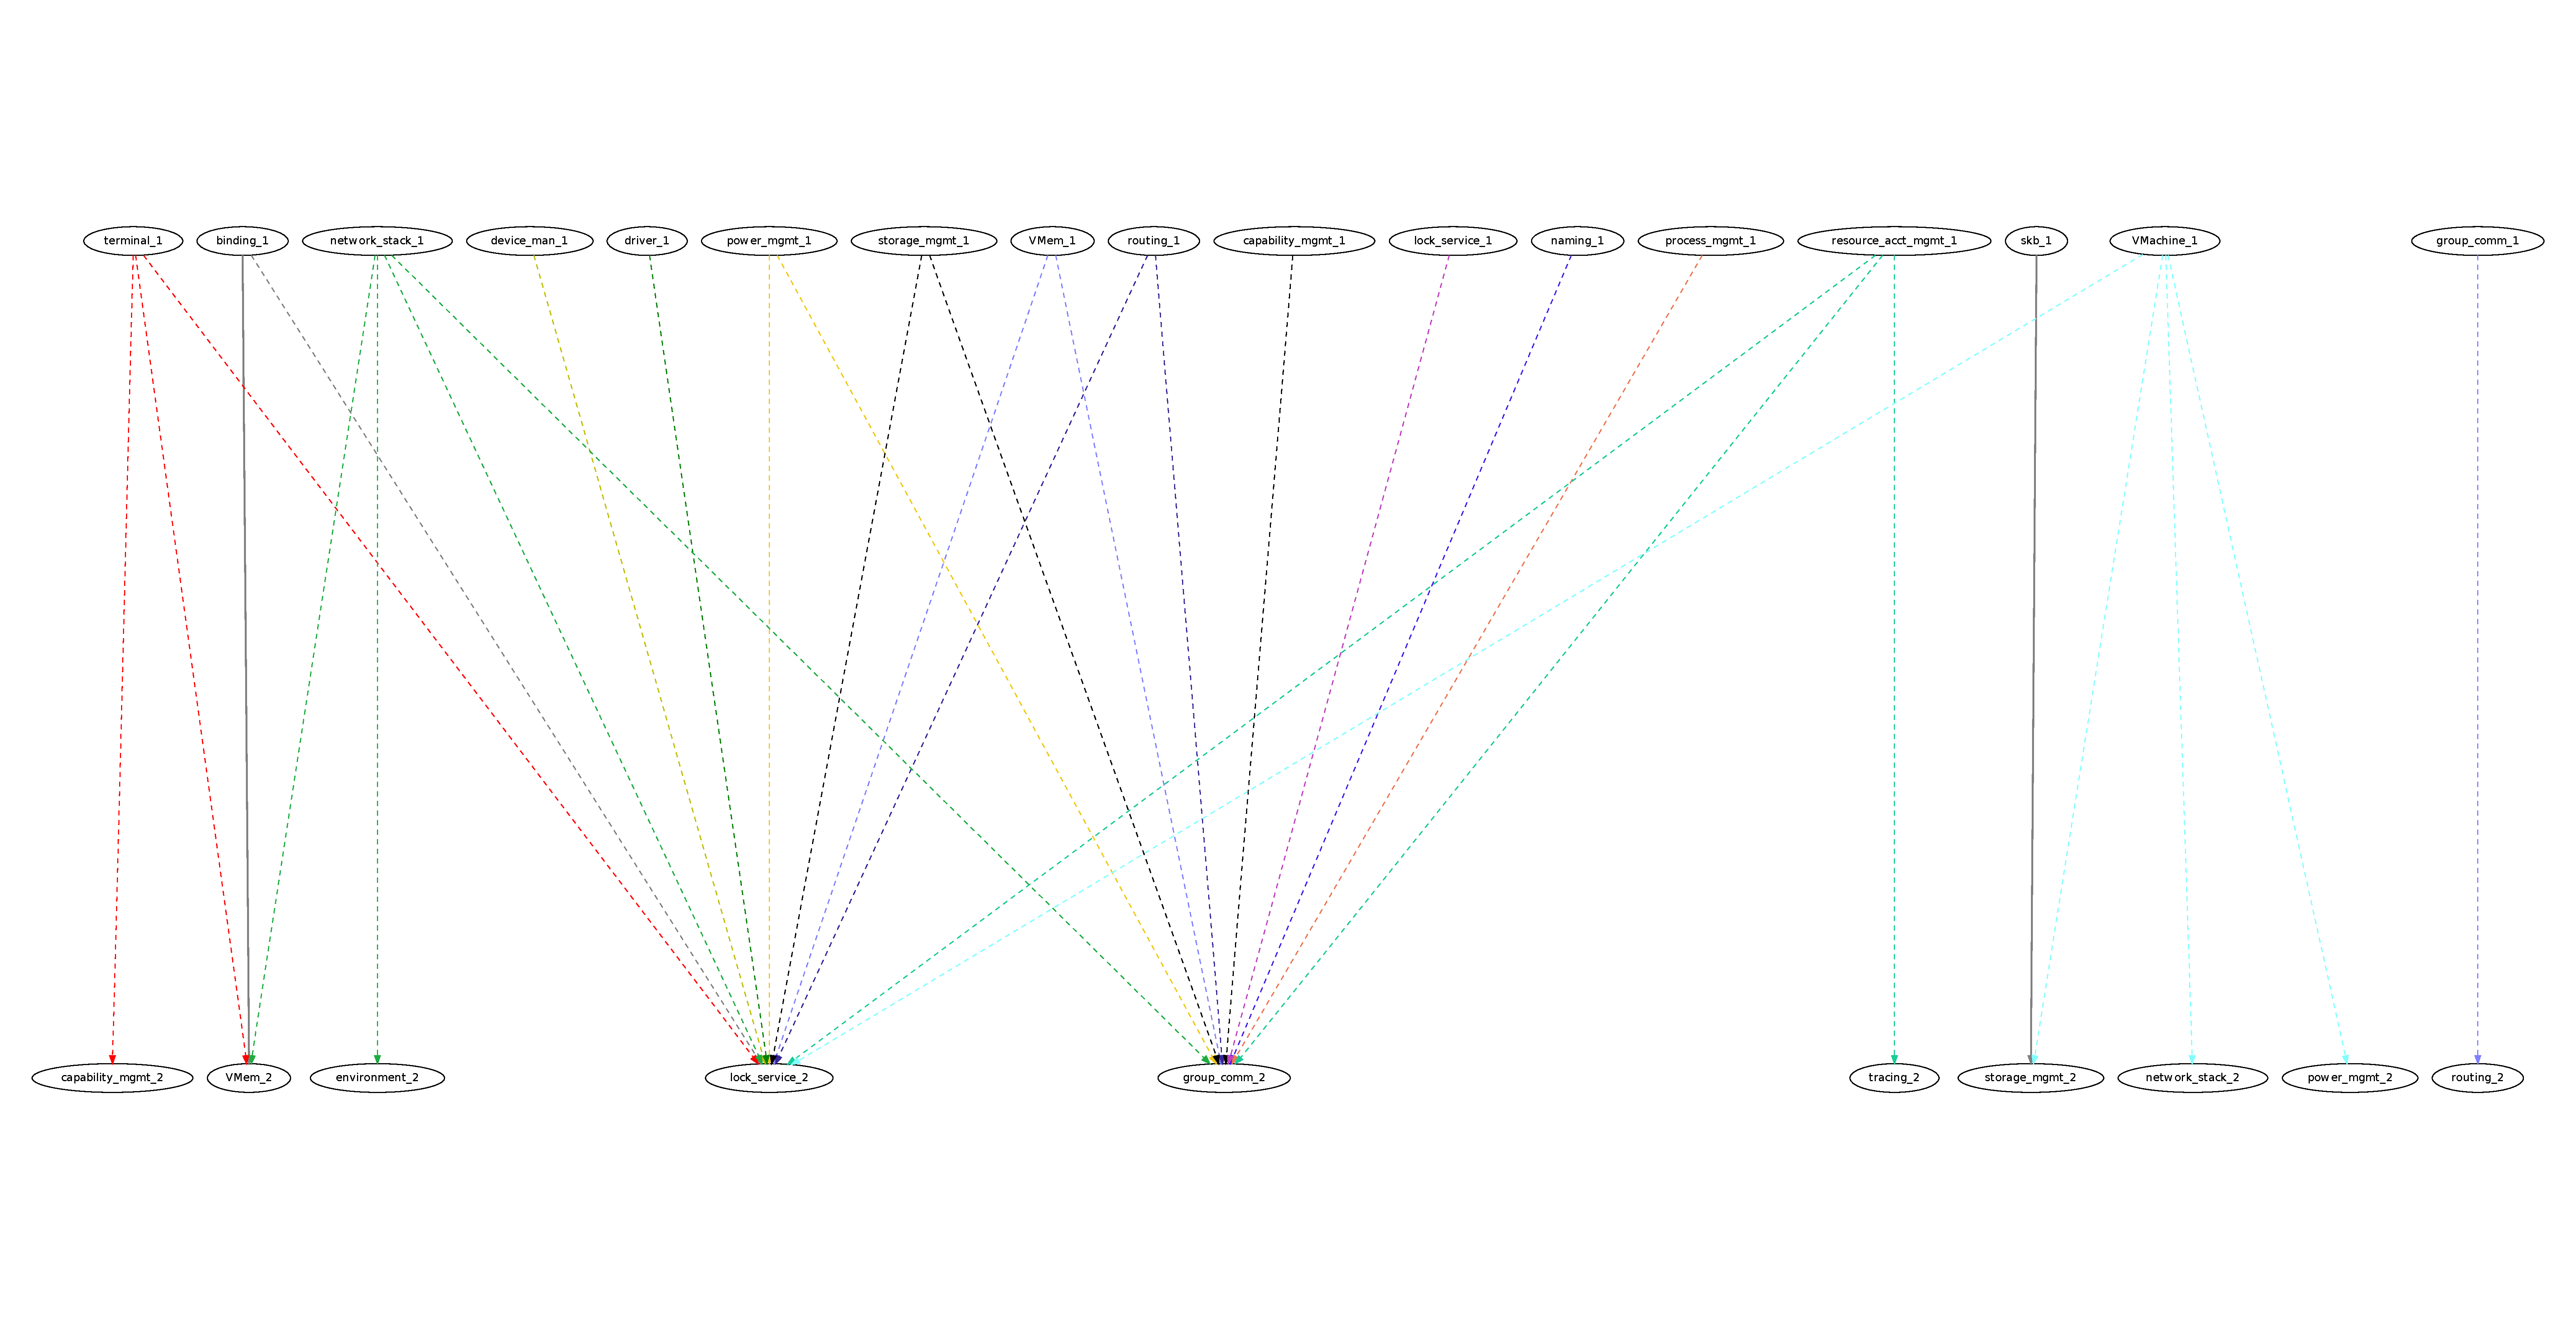
\includegraphics[angle=270,scale=0.15]{dep2-i-dot.pdf}
 \end{center}
 \caption{Subset of non-barrelfish implementation dependencies between OS
   services}\label{fig:dep2-i} 
\end{figure}

Discussion of these dependencies is presented below.

\subsection{Binding}

All services have a Barrelfish-specific dependency on the binding
service, since, if they are implemented as Barrelfish dispatchers,
they will require the binding service to make their interfaces
available to others, as well as to connect to and communicate with
other services.

The binding service itself requires endpoint capabilities for the communication
and therefore has a dependency on the capability management service.
It also needs to know about the cores and hardware support for
communication available in the system, and therefore has a dependency
on the SKB, which provides such information.

The binding service, besides providing poin-to-point connections, also
provides access to the group communication service and the routing
service for more complex communication, and therefore has a dependency
on both these services.  Communication also involves notifying and
scheduling dispatchers when messages arrive, so the binding service must
also make use of the process management service.


Finally, the implmentation of the binding service needs to set up
shared memory areas for the implementation of UMP, so needs to use the
virtual memory service.  Its impementation may also make use of
locking and synchronisation primitives, leading to a potential
dependency on the locking service.


\subsection{Capability Management}

Managing capabilities requires access to basic memory capabilities,
which are provided through the memory allocation service, leading to a
dependency on that service.  This service will also depend on the
virtual memory management service, since it will require control of
memory for management of metadata.

\subsection{Debugging}

The debugging service needs access to lower level services in order to
inspect and modify the system.  This includes: capability management
for access to system capabilities, threading to attach to and control
threads, process management to attach to and control processes
(dispatchers and domains), virtual memory service to inspect and
modify address spaces, memory mappings, etc.  The debugging service
will also use the SKB service to provide further information about the
system and its resources.

\subsection{Device Drivers}

Device drivers depend on the capability management service since they
need to manage and use capabilities to the hardware devices. Drivers
also use the memory allocation service since they need to manipulate
memory, for example, to use DMA and access device memory.   This also
requires the use of the virtual memory service.

Since drivers must react to system power events (e.g., to turn devices
on and off when the system suspends) they may also depend on the power
management service.

\subsection{Device Management}

The device management service works closely with the SKB since it
needs to find out (and register) information about devices in the
system. It may also depend on the power management service to
determine current power state and possibly inform drivers of changes
in the state.  

%% The device manager will likely be implemented as a multithreaded
%% service and may rely on the locking service for locking and synchronisation.

\subsection{Environment}

The environment service may use the principals service if provides
per-principal environments, and the process management service if it
provides per-process environements. 

\subsection{Group Communication}

The group communication service depends on the binding service to provide a
frontend interface, as well as to send individual messages.
The group communication service will also depend on the SKB to find out
information about the system (e.g., interconnect toplogy) to help
implement efficient message delivery (e.g., multicast trees).

Group communication is typically associated with consensus protocols,
and may therefore rely on a locking services. Alternatively, the group
communication service may be used by the locking service to implement
some synchronisation.

The service may require endpoints to implement the underlying
communication, and will then be dependent on the capability management service.
The service will typically also make use of the routing service to
send messages to group members.

\subsection{Locking}

The locking service interacts closely with the process management and
threading services since it must be able to suspend and resume
execution to correspond with blocking and signalling.

The locking service may depend on the group communication service to
implement consensus and other forms of synchronisation.


\subsection{Memory Allocation}

The memory allocation service requires capabilities to do memory
management in Barrelfish, so has a dependency on the capabiity
management service.

It may also depend on the SKB to find out about all the memory
resources in the system, and it may also act as a client of the
resource accounting and management service to provide it with
information about memory usage.

\subsection{Naming}

All services have a Barrelfish-specific dependency on the name
service, since, if they are implemented as Barrelfish dispatchers
then they will either need to register with it, or use it to find
other services that they depend on.

Depending on its implementation the naming service may use the group
communication service.

\subsection{Network Stack}

The network stack service requires access to NIC drivers to access the
network hardware.  It may also need to use the SKB to determine what
network hardware and drivers are available in the system.  

Depending on implementation details, the network stack may also need
to use the virtual memory service to implement zero-copy mechanisms, etc.

\subsection{Power Management}

The power management service requires access to device drivers and the
device management service to monitor and control the power states of hardware.
It will also need to use the SKB to determine what devices to manage
in the system and what power management hardware is available.

The service may also need access to the the resource management service
to help make power management decisions. The power management service
may also need to manipulate capabilities for power management
hardware, in which case it will need access to the capability
management service.

Depending on its implementation it may also use the group
communication and locking services.

\subsection{Principals}

In Barrelfish the principals service will make use of capabilities to
implement access control, and will therefore require access to the
capability management service.

\subsection{Process Management}

The process management service will need access to the capability
management and virtual memory services in order to prepare and
manipulate process address spaces for execution. It will also work
closely with the threading service, to manage execution, and the
principals service, to provide processes with the appropriate caps for
access control.

The service may use the group communication service depending on how
it is implemented.

\subsection{Resource Accounting and Management}

The resource accounting and management service will use the various
other management and accounting services (power management, process
management, bus management, drivers, storage management) to determine
the state of the system and resource usage in the system.  It will
also use these services to change resource usage according to policy.

It will also both read from and write to the SKB.

In order to manage resource usage the resource management service may
need to manipulate caps, in which case it will use the capability
management service.

Depending on implementation it may also use the group communication and
locking services.

\subsection{Routing}

The routing service will require endpoint capabilities for communication
and therefore has a dependency on the capability management service.
It also needs to know about the cores and hardware support for
communication available in the system, and therefore has a dependency
on the SKB, which provides such information.

The routing service will both make use of the binding service for its
point-to-point connections, as well as be accessed through the binding
service, and thus has a strong dependency to it.

The routing service will use the SKB to determine the system topology.

It will likely also be implemented using locking and group
communication.

\subsection{Shell}

The shell service requires access to process management and threading
to start and control programs, it also requires access to the
environment service to provide programs with appropriate execution
environments, and allow manipulation of those environments. It uses
the principals service to determine and set up access control for the
programs it starts.  The storage management service is used to fetch
the code to execute, and the terminal service is used for input and output.

\subsection{SKB}

The SKB relies on the storage management service to read its startup
files, and possibly store its knowledge base.

\subsection{Storage Management}

The storage management service needs access to appropriate storage
hardware (e.g., disk). 

It will also use the virtual memory service if it implements zero-copy
features and needs to manipulate shared memory buffers. It may need to
use the SKB to determine what devices are available.

The service may also require access to the
principals service for access control, however this depends on the
chosen design.
% or the user may authenticate via the principals service and receive
% the apropriate caps which it then uses to access the storage services.

Depending on implementation it may also use the using locking and group
communication services.

\subsection{Terminal}

The terminal service will need to use drivers to access the input and
output hardware.

Depending on implementation it may use the virtual memory and
capability management services to provide access through a
framebuffer.

The implementation will likely use locking, and may require the SKB to
determine what interaction devices are available.

\subsection{Threading}

The threading service closely cooperates with the process management
service.  
% because the pm services provides dispatcher functionality
It also needs to manage the memory accessible by threads and
uses the capability management and virtual memory management services
for this.

It may also cooperate closely with the locking service to suspend and
resume threads as part of the locking mechanism implemententations.

\subsection{Tracing}

The tracing service is not directly dependent on other services (other
than binding and naming).

Any service may use the tracing service to log trace points.  We have
not represented these dependencies explicitly.

\subsection{Virtual Machine Monitor}

The virtual machine monitor service uses the capability management,
memory allocation, virtual memory management, and process management
services to provide a virtual machine environment to a guest OS.  It
also uses the driver and device menagement services to provide access
to  hardware devices. 

It may also use the storage managment and network stack services to
virtualise disk and network traffic. The power management service may
be used to allow power management of and by the virtual machine.  
The SKB may be used to determine which system resources to provide to
the virtual machine.

Its implementation is likely to use locking.


\subsection{Virtual Memory}

The virtual memory service uses the capability management and memory
allocation services to help manage the virtual memory mappings and
address spaces.  The SKB is used to determine the available memory
resources in the system.

Paging will use an appropriate disk driver, and may require access to
a storage management service.

The implementation of virtual memory management is likely to use
locking and group communication.


\section{Status}

Some of the services discussed above have already been implemented.
In many cases the implementation has been a simple prototype
implementation, where the basic functionality has been implemented,
but without regard to issues such as scalability, and also, without
attempting to dynamically configure or alter functionality based on
information about the system gathered at runtime (e.g., from the SKB).

In this section we provide an overview of the current status of each
service.  A service's status can be: 
\begin{description}
  \item[N]: Does not exist
  \item[P]: Exists as a prototype
  \item[E]: Fully featured implementation
  \item[D]: Scalable, distributed, implementation
\end{description}

We also provide an overview of the development priority of services.
The priorities relate to the goal of developing a complete OS and an
environment and tools for developing complete OSes.
The priorities are: 
\begin{description}
  \item[High]: This service must exist before more of the system can
    be built, or it is a bottleneck and must be implemented in a
    scalable way. It is a core building block.
  \item[Medium]: Some services rely on this, so it has some priority.
    Availability of the service may also help the usability of the
    system. It is a useful building block.
  \item[Low]: Hardly any services depend on this, so lack of it will
    not stand in the way of developing a system.
\end{description}


The status of the services is as follows:

\begin{tabularx}{\textwidth}{|l|c|c|X|}
\hline
Service & Status & Priority & Comment \\
\hline
Binding & E & High & implemented by combination of monitor, barrelfish
library, and flounder stubs. \\ 
\hline
Capability Management & P & High & implemented by combination of monitor and
barrelfish library. The revoke fnctionality is not implemented. \\ 
\hline
Debugging & N & Low & \\ 
\hline
Device Driver & E & Medium & existing drivers: serial, pci, e1000 \\ 
\hline
Device Management & P & Medium & implemented by pci driver and skb \\ 
\hline
Environment & P & Low & implemented by barrelfish library and spawnd
dispatcher \\
\hline
Group Communication & N & Medium \\ 
\hline
Locking & P & High & ??? how is locking/synchronisation currently done???\\ 
\hline
Memory Allocation & P & High & implemented by memory server domain. No
ability to free or reuse memory. \\ 
\hline
Naming & E & High & implemented by chips domain. \\ 
\hline
Network Stack & P & Medium & implemented as library. can be used by only 1
dispatcher at a time. It is based on LWIP. \\ 
\hline
Power Management & N & Low & \\ 
\hline
Principals & N & Medium & \\ 
\hline
Process Management & P & High & implemented by combination of spawnd domain,
monitor, and barrelfish library. \\ 
\hline
Resource Accounting and Management & N & Low & \\ 
\hline
Routing & N & Medium & \\ 
\hline
Shell & P & Low & implemented by fish domain.\\ 
\hline
SKB & E & Medium & implemented by skb domain. \\ 
\hline
Storage Management & P & Medium & implemented by combination of ramfsd domain,
and vfs library.\\  
\hline
Terminal & N & Medium & there is some code to handle this in lib
barrelfish. \\ 
\hline
Threading & E & High & implemented by barrelfish library. \\ 
\hline
Tracing & E & Medium & implemented by tracing library. \\ 
\hline
Virtual Machine Monitor & P & Medium & implemented by vmmkit domain. \\ 
\hline
Virtual Memory & P & High & implemented by monitor and barrelfish library (???).
No support for paging, unmap, or fault handling. \\ 
\hline
\end{tabularx}





%% \begin{figure}[hbt]
%%  \begin{center}
%%  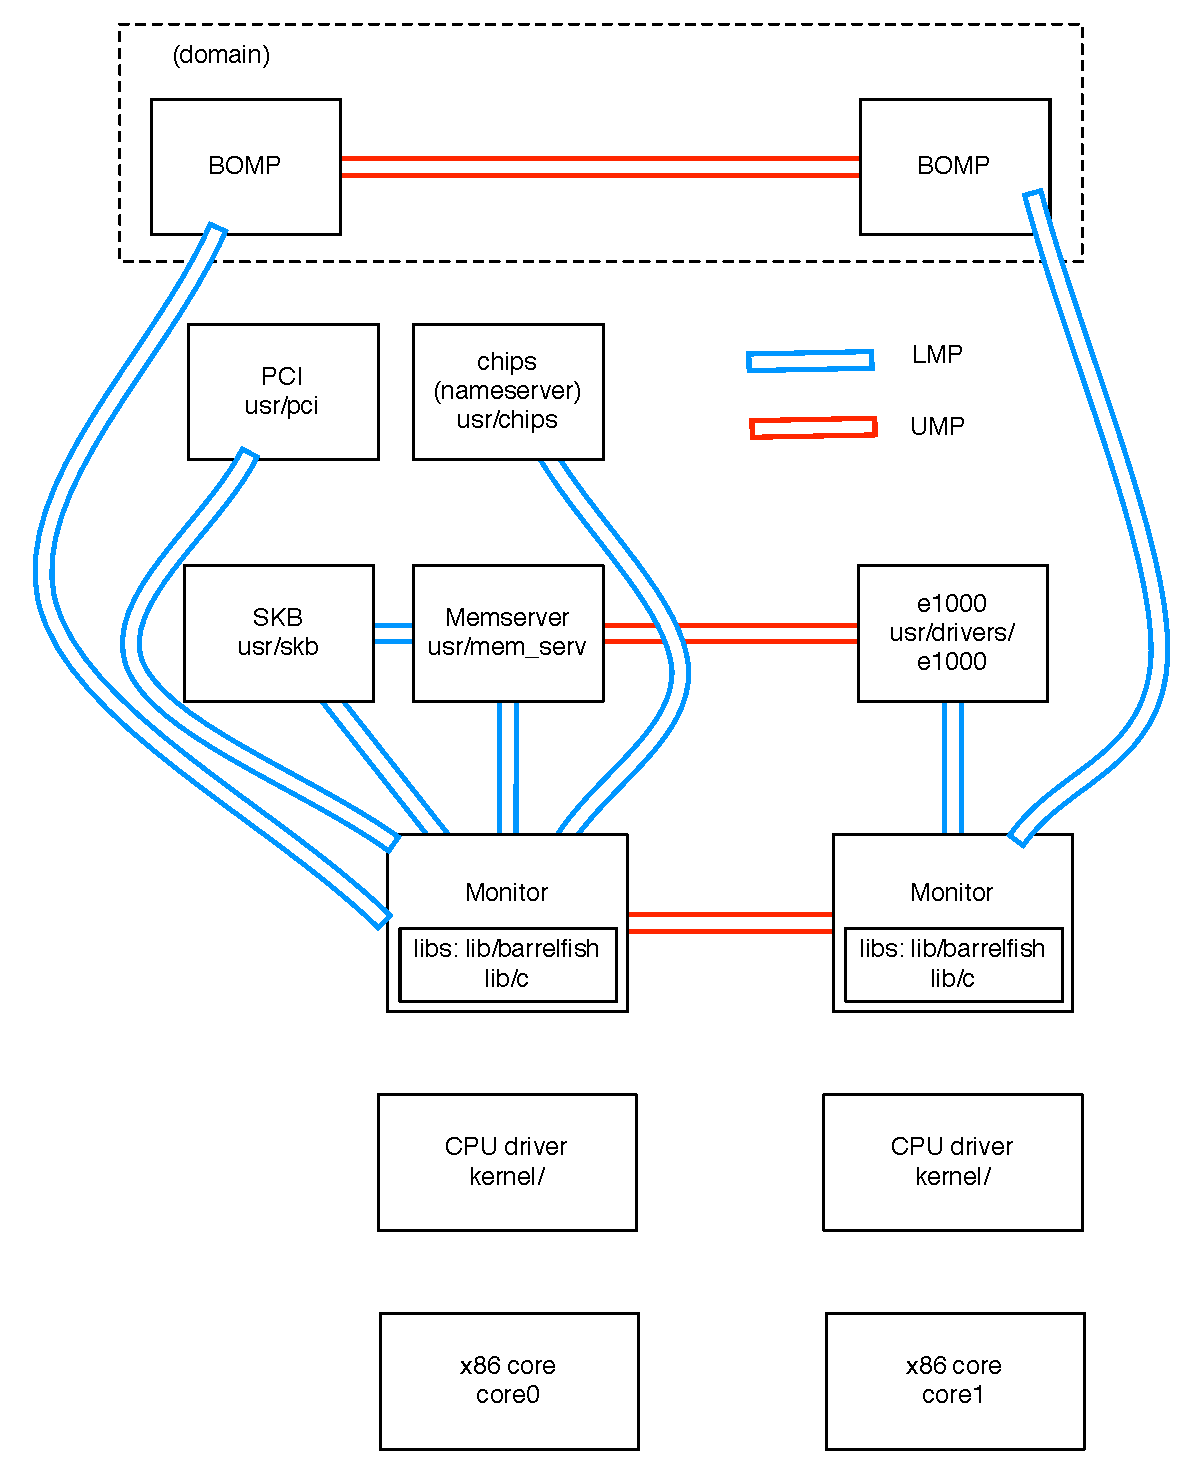
\includegraphics[width=0.5\columnwidth]{os-arch.pdf}
%%  \end{center}
%%  \caption{High level overview of the Barrelfish OS architecture}\label{fig:os-arch}
%% \end{figure}


%%%%%%%%%%%%%%%%%%%%%%%%%%%%%%%%%%%%%%%%%%%%%%%%%%%%%%%%%%%%%%%%%%%%%%%%%%%%%%%%
\bibliographystyle{abbrvnat}
\bibliography{paper}

\end{document}
